% !TeX root = ../main.tex

\section{Introduction}
\subsection{Recommender Systems Overview}
\begin{frame}[t]
    \frametitle{Recommender Systems Overview}
    \vspace{-1cm}
    \begin{itemize}
        \item<1->What is a recommender system and what does it do?\\
        \only<1-6>{
            \begin{enumerate}
                \item<2-> Predict how much a user may like a certain item
                \item<3-> Compose a list of N best items for a user
                \item<4-> Compose a list of N best users for a specific item
                \item<5-> Explain to the users why these items are recommended them
                \item<6-> Adjust the prediction and recommendation based on user's and
                other people feedback
            \end{enumerate}
        }
        \item<7->Why we need a recommender system?
        \only<7>{
            \begin{figure}
                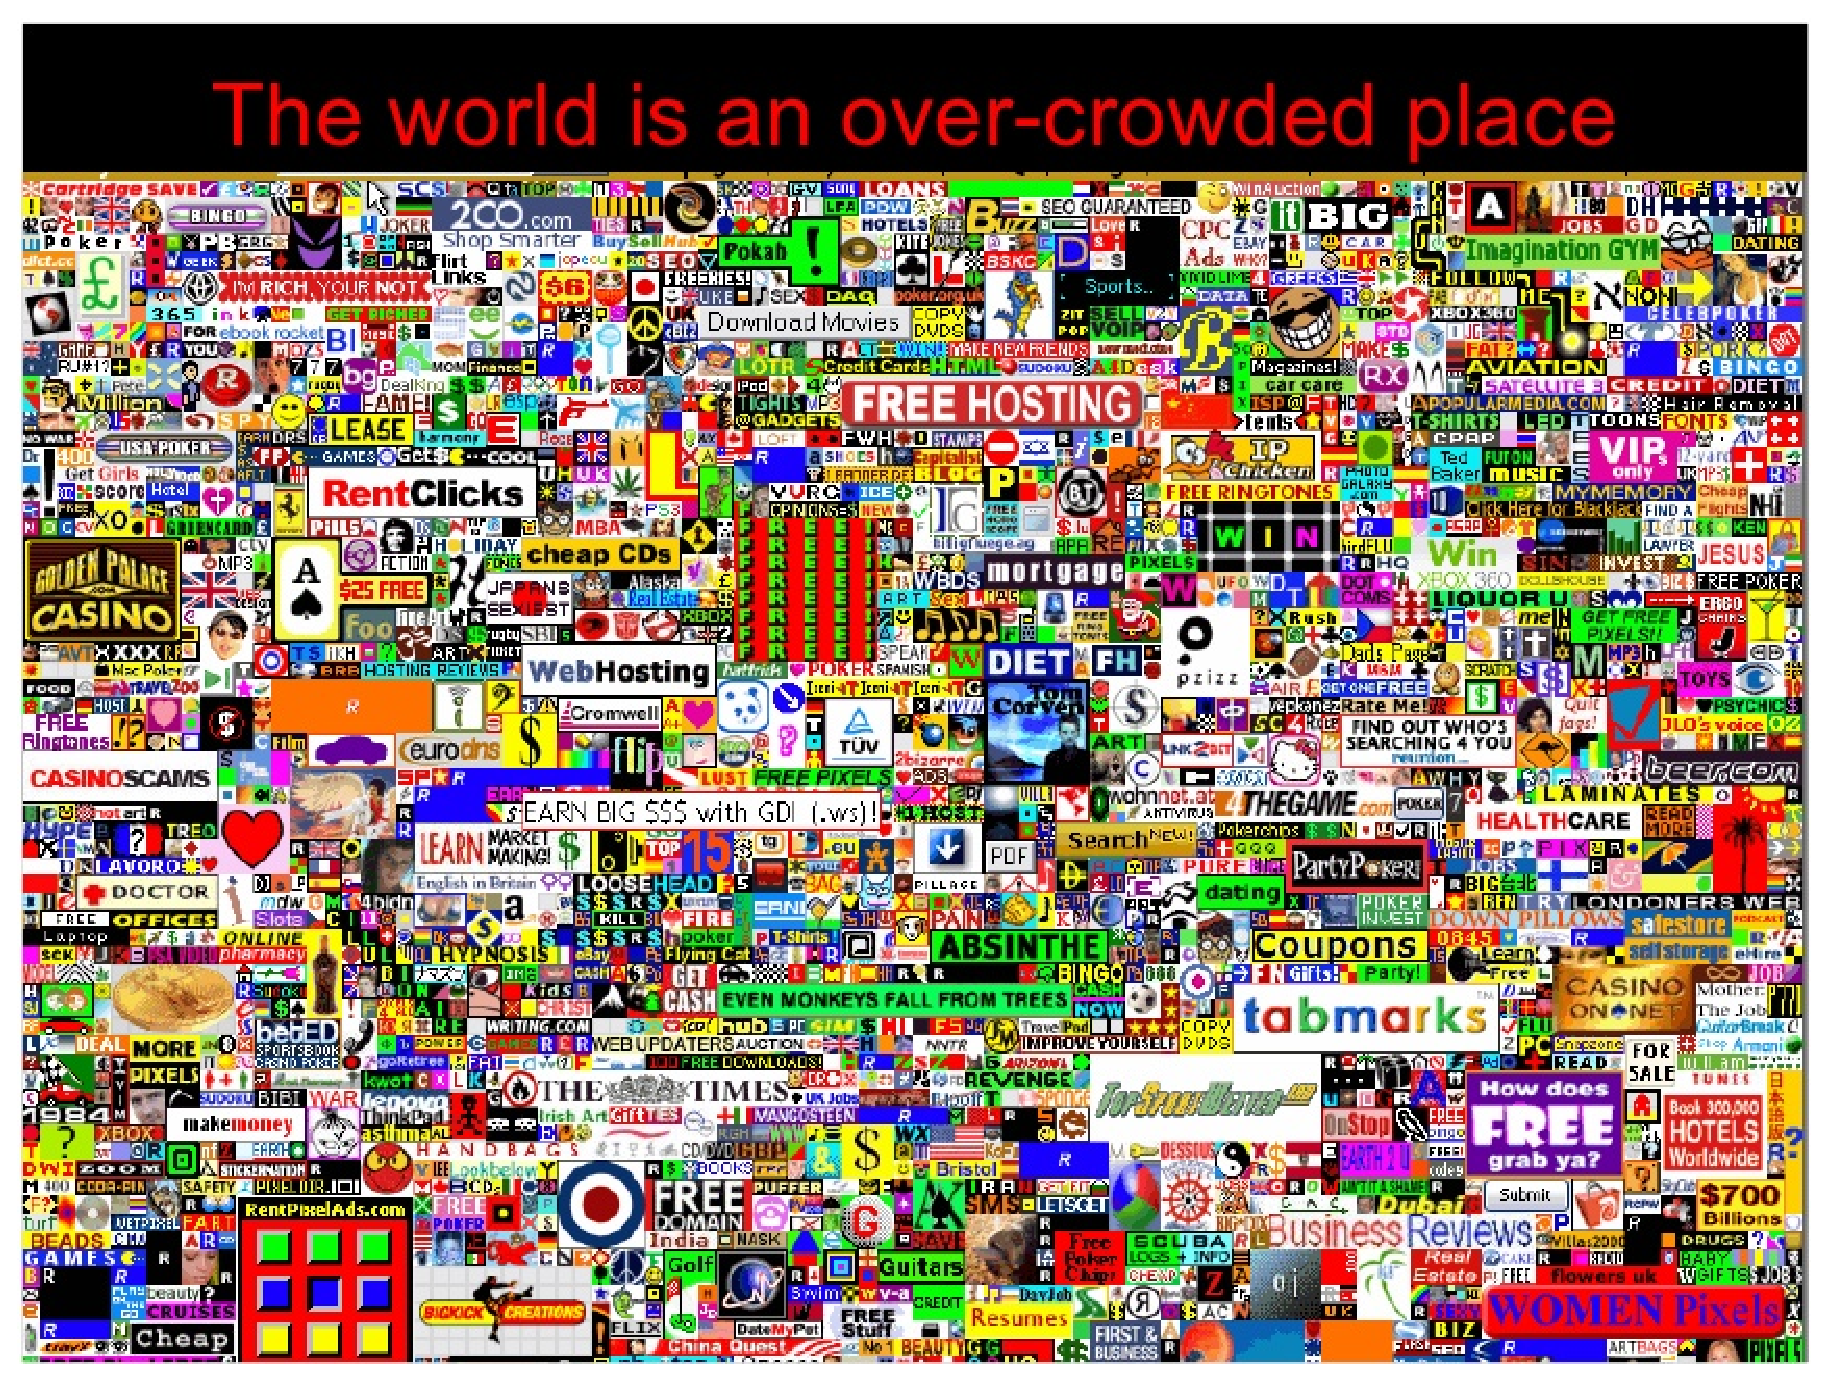
\includegraphics[width=0.7\textwidth,height=0.65\textheight]{overcrowded.eps}
            \end{figure}
        }
        \item<8->How we build a recommender system?
        \only<8-12>{
            \begin{enumerate}
                \item<9->\textbf{Collaborative Filtering}
                    \begin{itemize}
                        \item Neighborhood-based
                        \item Model-based
                    \end{itemize}
                \item<10->\textbf{Content-based}
                \item<11->\textbf{Knowledge Based}
                \item<12->\textbf{Hybrid}
            \end{enumerate}
        }
    \end{itemize}
\end{frame}
\subsection{Motivation}
\begin{frame}[t]
    \frametitle{Motivation}
    \centering
    \underline{\textbf{Problems with collaborative filtering}}
    \vspace{0.5cm}
    \begin{enumerate}
        \item \textbf{Scale}
        \begin{itemize}
            \item New users and items enter a recommendation platform everyday.
        \end{itemize}
        \item \textbf{Sparse data}
        \begin{itemize}
            \item A user has rated only one item or an item has been rated only once.
        \end{itemize}
        \item \textbf{Cold-Start}
        \begin{itemize}
            \item New users and items have no history.
        \end{itemize}
   \end{enumerate}
\end{frame}
\subsection{Approach}
\begin{frame}[t]
    \frametitle{Approach}
    \centering
    \underline{\textbf{Objectives}}
    \vspace{1cm}
    \begin{enumerate}
        \item Explain the Neighborhood-based Collaborative Filtering
        \item Propose the Recursive Nearest Neighbors Algorithm
        \item Present the Experimental results on the Epinions data set.
    \end{enumerate}
\end{frame}
